
\begin{block}{Results}
    \begin{figure}[h]
        \centering
        \fbox{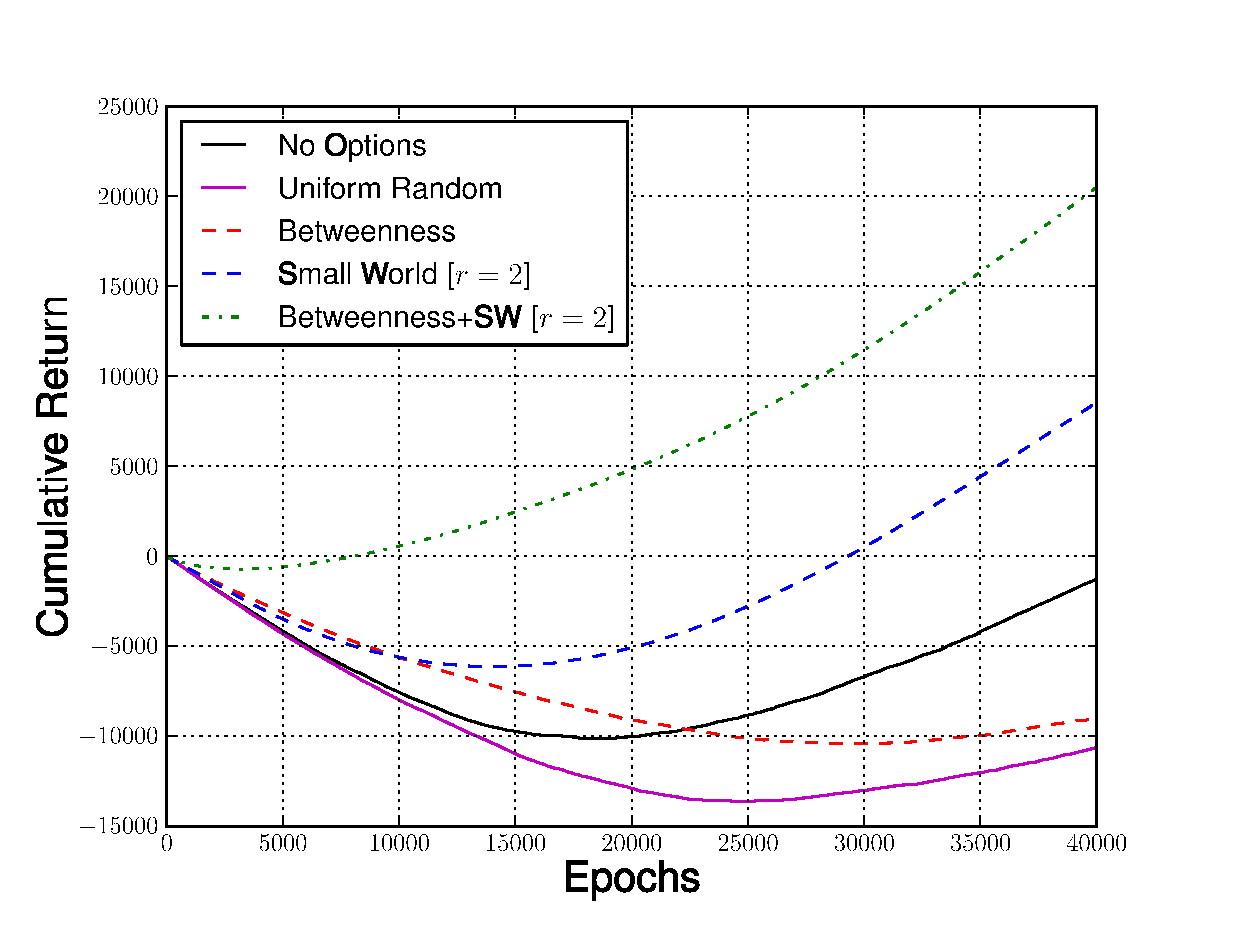
\includegraphics[height=4in]{figures/rooms-algos-200}}
        \label{fig:rooms-performance}
        \caption{Rooms: Cumulative Return (with 200 options)}
    \end{figure}

    \vskip-4ex
    % Table
    \begin{columns}
        \begin{column}{.45\textwidth}
            \begin{table}
              \centering
              \small
              \begin{tabular}{ l r r } %{@{} p{.25\linewidth} p{.2\linewidth} p{.2\linewidth} p{0.2\linewidth} }
                \toprule 
                Scheme & \multicolumn{2}{c @{}}{Options (40,000 epochs)}  \\
                \cmidrule(l){2-3}
                                & {200}             & {400}  \\
                \toprule
                None            & -31.82         & -31.82   \\
                \addlinespace                            
                $P_0$           & -31.23         & -32.90   \\  
                \addlinespace                            
                Betw.           & -18.28         & -24.38   \\
                \addlinespace                                  
                $P_4$           & {\bf -14.24}   & {\bf -7.55}    \\
                \bottomrule
              \end{tabular}
              \caption{Arb. Nav.: Cumulative Return}
            \end{table}
        \end{column}
        \begin{column}{.45\textwidth}                
            \begin{table}
              \centering
              \small
              \begin{tabular}{ l r r } %{@{} p{.25\linewidth} p{.2\linewidth} p{.2\linewidth} p{0.2\linewidth} }
                \toprule 
                Scheme & \multicolumn{2}{c @{}}{Options (40,000 epochs)}  \\
                \cmidrule(l){2-3}
                                        & {100}         & {200}            \\ %& {400}    \\
                \toprule                                    
                None                    & -16.90        & -16.90           \\ %& -3043.60 \\
                \addlinespace                                                   %          
                $P_0$                   & -17.68         & -18.83           \\ %& -8304.05 \\  
                \addlinespace                                                   %           
                Betw.                   & {\bf 80.59}   & {\bf 80.48}      \\ %& 14841.15 \\
                \addlinespace                                                   %   
                $P_{0.75}$                 & -7.55          & 0.66             \\ %& 22605.01 \\
                % \addlinespace                                                %     
                % Betw. + \\$P_{0.75}$      & 12.69          & 15.12        \\ %& {\bf 23168.17} \\
                \bottomrule
              \end{tabular}
              \caption{Taxi: Cumulative Return}
            \end{table}
        \end{column}
    \end{columns}

    % Comments
    \begin{itemize}
        \item Experiments were run for 40,000 epochs using MacroQ. We compared
            options generated using a bottleneck based method (betweenness),
            randomly distributed options ($P_0$), and small world options ($P_{r
            > 0}$).
        \item Bottleneck-based methods have a natural advantage in the Taxi
            domain, as goal states coincide with bottleneck states (the {\tt
            pick-up} and {\tt put-down} actions). 
        \item Small-world options do very well on free-navigation tasks (Rooms
            or Arbitrary Navigation), even in the presence of bottlenecks
            (Rooms). Combining bottleneck-based options and small world
            options can outperform both (Rooms).
    \end{itemize}
\end{block}

\vfill
\begin{block}{Role of the Exponent $r$ (Rooms)}
    \begin{columns}
        \begin{column}{.49\textwidth}
            \begin{figure}[h]
                \centering
                \fbox{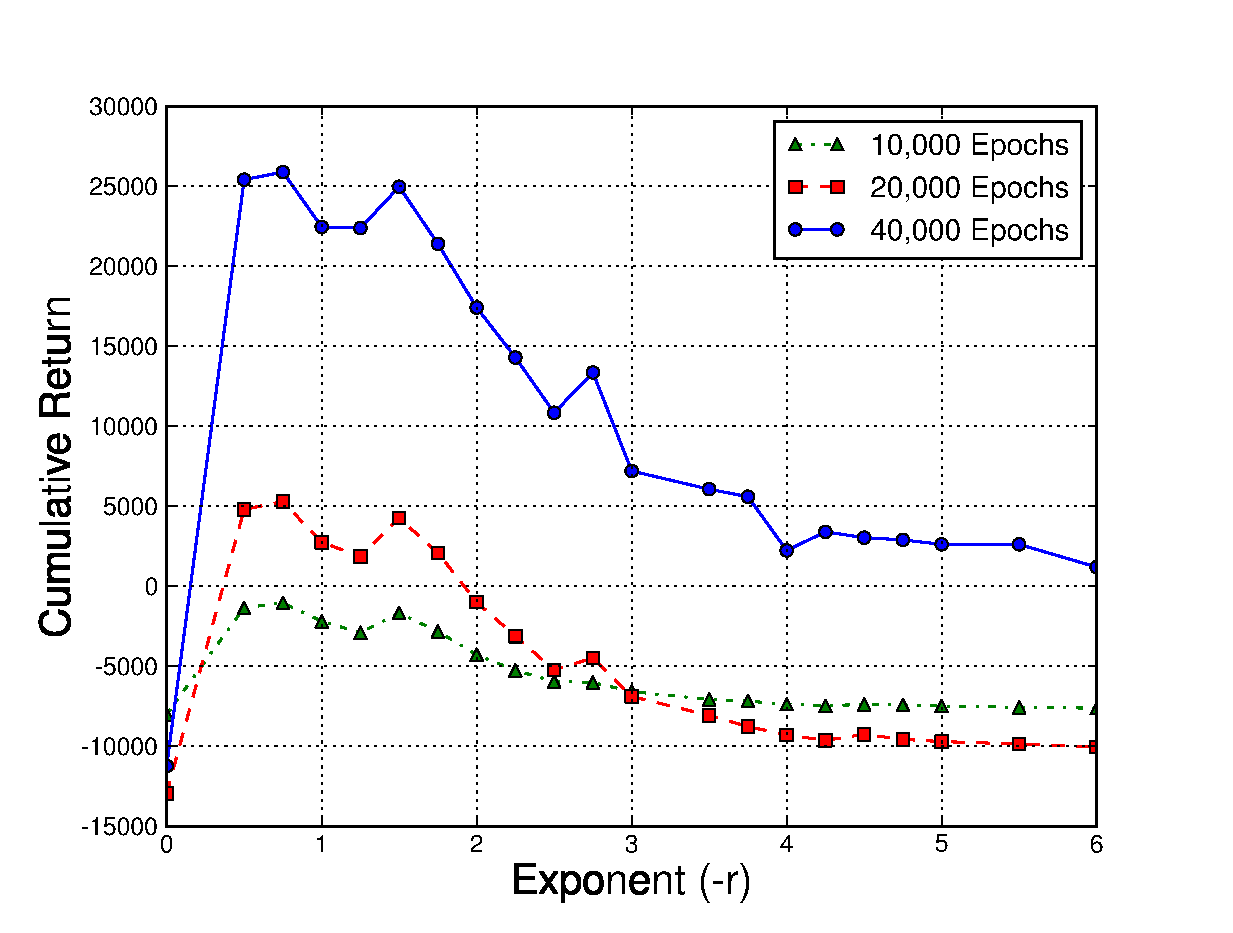
\includegraphics[height=3in]{figures/rooms-exp}}
                \label{fig:rooms-exponent}
                %\caption{Rooms}
            \end{figure}
        \end{column}
        \begin{column}{.39\textwidth}                
            \begin{itemize}
                \item The basic structure of the the Rooms state spaces is 2D,
                    yet exponents around 1 perform optimally.  This difference
                    is likely due to obstacles (walls).
                \item The existance of a maximal value for the exponent, as well
                    the behaviour for exponents greater than it, matches what is
                    seen in the social networks scenario.
            \end{itemize}
        \end{column}
    \end{columns}
\end{block}

\vfill
\begin{block}{Conclusions}
    \begin{itemize}
        \item We give an algorithm to generate a random collection of options
            $\options$ such that any ``task'' in an MDP can be performed in
            $O( ( \log |\states| )^2 )$ decisions.
        \item We find that these options significantly outperform
            bottleneck-based options and purely random options.
    \end{itemize}
\end{block}

\vfill
\begin{block}{Future Work}
    \begin{itemize}
        \item By using `cheaply' learnt policies could the total training time
            for small world options compare to say that for the case of
            betweenness?
        \item Given the loose conditions for the theorem to hold, could function
            approximators be used inplace of the complete MDP?
        \item Could the bounded number of decisions required translate to any
            theoretical guarantees on faster convergence?
    \end{itemize}
\end{block}
